\documentclass{article}
\usepackage{physics}
\usepackage{graphicx}
\usepackage{caption}
\usepackage{amsmath}
\usepackage{bm}
\usepackage{framed}
\usepackage{authblk}
\usepackage{empheq}
\usepackage{amsfonts}
\usepackage{esint}
\usepackage[makeroom]{cancel}
\usepackage{dsfont}
\usepackage{centernot}
\usepackage{mathtools}
\usepackage{bigints}
\usepackage{amsthm}
\theoremstyle{definition}
\newtheorem{defn}{Definition}[section]
\newtheorem{prop}{Proposition}[section]
\newtheorem{rmk}{Remark}[section]
\newtheorem{thm}{Theorem}[section]
\newtheorem{exmp}{Example}[section]
\newtheorem{prob}{Problem}[section]
\newtheorem{sln}{Solution}[section]
\newtheorem*{prob*}{Problem}
\newtheorem{exer}{Exercise}[section]
\newtheorem*{exer*}{Exercise}
\newtheorem*{sln*}{Solution}
\usepackage{empheq}
\usepackage{tensor}
\usepackage{xcolor}
%\definecolor{colby}{rgb}{0.0, 0.0, 0.5}
\definecolor{MIT}{RGB}{163, 31, 52}
\usepackage[pdftex]{hyperref}
%\hypersetup{colorlinks,urlcolor=colby}
\hypersetup{colorlinks,linkcolor={MIT},citecolor={MIT},urlcolor={MIT}}  
\usepackage[left=1in,right=1in,top=1in,bottom=1in]{geometry}

\usepackage{newpxtext,newpxmath}
\newcommand*\widefbox[1]{\fbox{\hspace{2em}#1\hspace{2em}}}

\newcommand{\p}{\partial}
\newcommand{\R}{\mathbb{R}}
\newcommand{\C}{\mathbb{C}}
\newcommand{\lag}{\mathcal{L}}
\newcommand{\nn}{\nonumber}
\newcommand{\ham}{\mathcal{H}}
\newcommand{\M}{\mathcal{M}}
\newcommand{\I}{\mathcal{I}}
\newcommand{\K}{\mathcal{K}}
\newcommand{\F}{\mathcal{F}}
\newcommand{\w}{\omega}
\newcommand{\lam}{\lambda}
\newcommand{\al}{\alpha}
\newcommand{\be}{\beta}
\newcommand{\x}{\xi}

\newcommand{\G}{\mathcal{G}}

\newcommand{\f}[2]{\frac{#1}{#2}}

\newcommand{\ift}{\infty}

\newcommand{\lp}{\left(}
\newcommand{\rp}{\right)}

\newcommand{\lb}{\left[}
\newcommand{\rb}{\right]}

\newcommand{\lc}{\left\{}
\newcommand{\rc}{\right\}}


\newcommand{\V}{\mathbf{V}}
\newcommand{\U}{\mathcal{U}}
\newcommand{\Id}{\mathcal{I}}
\newcommand{\D}{\mathcal{D}}
\newcommand{\Z}{\mathcal{Z}}

%\setcounter{chapter}{-1}


\usepackage{enumitem}



\usepackage{subfig}
\usepackage{listings}
\captionsetup[lstlisting]{margin=0cm,format=hang,font=small,format=plain,labelfont={bf,up},textfont={it}}
\renewcommand*{\lstlistingname}{Code \textcolor{violet}{\textsl{Mathematica}}}
\definecolor{gris245}{RGB}{245,245,245}
\definecolor{olive}{RGB}{50,140,50}
\definecolor{brun}{RGB}{175,100,80}

%\hypersetup{colorlinks,urlcolor=colby}
\lstset{
	tabsize=4,
	frame=single,
	language=mathematica,
	basicstyle=\scriptsize\ttfamily,
	keywordstyle=\color{black},
	backgroundcolor=\color{gris245},
	commentstyle=\color{gray},
	showstringspaces=false,
	emph={
		r1,
		r2,
		epsilon,epsilon_,
		Newton,Newton_
	},emphstyle={\color{olive}},
	emph={[2]
		L,
		CouleurCourbe,
		PotentielEffectif,
		IdCourbe,
		Courbe
	},emphstyle={[2]\color{blue}},
	emph={[3]r,r_,n,n_},emphstyle={[3]\color{magenta}}
}






\begin{document}
\begin{framed}
	\noindent Name: \textbf{Huan Q. Bui}\\
	Course: \textbf{8.309 - Classical Mechanics III}\\
	Problem set: \textbf{\#4}
\end{framed}
	
	

\noindent \textbf{1. A Heavy Symmetric Top.}
\begin{enumerate}[label=(\alph*)]
	\item In the body axes, the $z_\text{body}$-torque component is zero. The only torque components are therefore in the $x_\text{body}$ and $y_\text{body}$ axes. The torque vector is always along the ``dotted'' axis which is a line rotated by the (Euler) angle $\phi$ from the inertial $x$ axis. The magnitude of this vector is $mgR\sin\theta$, and the corresponding projections onto the $x_\text{body}$ and $y_\text{body}$ axes take the values $mgR\sin\theta\cos\psi$ and $-mgR \sin\theta\sin\psi$, respectively. Thus,
	\begin{align*}
	\vec{\tau} = 
	\begin{pmatrix}
	mgR\sin\theta \cos\psi\\
	-mgR\sin\theta \sin\psi\\
	0
	\end{pmatrix}
	\end{align*}
 	
%	The kinetic energy in terms of the principal angles is
%	\begin{align*}
%	T = \f{I_1}{2}(\omega_1^2 + \omega_2^2) + \f{I_3}{2}\omega_3^2
%	\end{align*}
%	Using the relations
%	\begin{align*}
%	\omega_{1} &= \dot\phi \sin\theta\sin\psi + \dot\theta \cos\psi  \\
%	\omega_{2} &= \dot\phi \sin\theta \cos\psi - \dot\theta \sin\psi \\
%	\omega_{3} &= \dot\phi \cos\theta + \dot\psi
%	\end{align*}
%	and the fact that the potential has the form
%	\begin{align*}
%	V = mgR \cos\theta,
%	\end{align*}
%	we find the general Lagrangian in terms of the Euler angles to be 
%	\begin{align*}
%	\lag = \f{I_1}{2}\lp \dot\theta^2 + \dot\phi^2\sin^2\theta  \rp + \f{I_3}{2}\lp \dot\psi + \dot\phi\cos\theta \rp^2 - mgR\cos\theta.
%	\end{align*}
%	From here, the components of the torque vector in terms of the Euler angles are simply 
%	\begin{align*}
%	&\boxed{p_\phi = \f{\p \lag}{\p \dot\phi} = (I_1\sin^2\theta + I_3 \cos^2\theta)\dot\phi + I_3\cos\theta \dot\psi = (I_1\sin^2\theta + I_3 \cos^2\theta)\dot\phi + I_3\cos\theta \omega'}\\
%	&\boxed{p_\theta = \f{\p \lag}{\p \dot\theta} = I_1\dot\theta = 0}\\
%	&\boxed{p_\psi = \f{\p \lag}{\p \dot\psi} = I_3( \cos\theta \dot\phi + \dot\psi ) = I_3( \cos\theta \dot\phi + \omega' )}
%	\end{align*}
%	where we have used the facts that $\dot\theta = 0$ and $\omega' \equiv \dot\psi$.
%	
	\item There are two angular velocities associated with the motion of the top: precession about the inertial vertical axis $z_I$ and rotation about the top about its principal $z$ axis. The latter is already defined by the problem: $\boxed{\omega' = \dot\psi}$. The only angular velocity is $\Omega$, and in terms of the Euler angles it is $\boxed{\Omega = \dot\phi}$.\\
	
%	Luckily, we have done this in Problem Set \#3. In general, 
%	\begin{align*}
%	\omega_x &= \dot\theta \cos\phi + \dot\psi \sin\theta\sin\phi  \\
%	\omega_y &= \dot\theta \sin\phi - \dot\psi \sin\theta\cos\phi\\
%	\omega_z &= \dot\psi \cos\theta  + \dot\phi.
%	\end{align*}
%	Putting in what we know about the setup of this problem ($\dot\theta = 0, \dot\phi = \omega'$, $\omega_z = \Omega$), we find 
%	\begin{align*}
%	&\boxed{\omega_x = \omega' \sin\theta\sin\phi}  \\
%	&\boxed{\omega_y = -\omega'\sin\theta\cos\phi}\\
%	&\boxed{\Omega = \omega'\cos\theta  + \dot\phi}
%	\end{align*}
	To see why $\omega' \equiv \dot\psi$ is constant in time, we recall from lecture that
	\begin{align*}
	\omega' = \dot\psi = \f{p_\psi}{I_3} - \f{(p_\phi - p_\psi\cos\theta)\cos\theta}{I_1\sin^2\theta}.
	\end{align*}
	Observe that $p_\psi$ and $p_\phi$ are conserved quantities since $\psi, \phi$ are cyclic coordinates and that $\dot\theta= 0$ as required by the problem. Therefore, $\dot\psi$ is a combination of constants in time and is thus constant in time. 
	
	
	\item Since $\theta = 0$ and $\dot\theta = 0$ initially, the energy of the top is simply the rotational energy about the vertical axis (body and inertial are now aligned) and the gravitational potential.
	\begin{align*}
	E = \f{1}{2}I_3 \omega_3^2 + Mgl.
	\end{align*} 
	The effective potential at any angle may therefore be written as 
	\begin{align*}
	V_\text{eff}(u) = (1-u^2)\lb -\f{2E I_3 - p_\psi^2}{2I_1 I_3} + \f{mgR}{I_1}u \rb + \f{1}{2}\lp \f{p_\phi - p_\psi u}{I_1} \rp^2.
	\end{align*}
	Let 
	\begin{align*}
	a = \f{p_\psi}{I_1}, \quad b = \f{p_\phi}{I_1}, \quad \al = \f{2E - I_3 \omega_3^2}{I_1} = \f{2E I_3 - p_\psi^2}{I_1I_3}, \quad \be = \f{2mgR}{I_1}.
	\end{align*}
	Then the effective potential simplifies to 
	\begin{align*}
	V_\text{eff}(u) = \f{1}{2}(1-u^2)( -\al + \be u ) + \f{1}{2}(b - au)^2.
	\end{align*}
	By the form of $E$, we immediately see that $\al = \be$. Moreover, since 
	\begin{align*}
	p_\phi = (I_1\sin^2\theta + I_3\cos^2\theta)\dot\phi + I_3\cos\theta\dot\psi \quad \text{and}\quad
	p_\psi = I_3(\dot\psi + \dot\phi \cos\theta),
	\end{align*}
	when we require $\theta \approx 0$ and $\cos\theta \approx 1$, we see that $p_\phi = p_\psi$. As a result, the effective potential becomes
	\begin{align*}
	V_\text{eff}(u) \propto \be(1-u^2)(u-1) + a^2(1-u)^2 = (1-u)^2 \lb -\be(1+u) + a^2 \rb.
	\end{align*} 
	Since we want $\cos\theta\approx 1$, we are interested in the case where $u=\cos\theta = 1$, which is a double root. In this case, the third root is given by 
	\begin{align*}
	u_3 = \f{a^2}{\be} - 1.
	\end{align*}
	For this cubic, we see that $V_\text{eff}\to -\infty$ when $u\to \infty$ and $V_\text{eff}\to \infty$ when $u\to -\infty$. Therefore, in order to achieve stability, the third root must be larger than the double root $u=1$, i.e., 
	\begin{align*}
	\f{a^2}{\be} - 1 > 1 \implies \f{a^2}{\be} = \f{1}{I_1} \f{I_3^2 \omega_c^2}{2mgR} > 2.
	\end{align*} 
	Thus, the critical/minimum value for the ``spinning'' angular velocity $\omega'$ is  
	\begin{align*}
	\boxed{\omega_c = 2{\f{\sqrt{mgR I_1}}{I_3}}}
	\end{align*}
	where the top will remain in its vertical spinning position whenever $\omega' > \omega_c$. In practice, no top will satisfy this condition for all possible $\omega'$s. One could make a top extremely light with extremely low center of mass, and so on. However, the top would be unphysical if $\omega_c$ were to vanish.  
\end{enumerate}

\noindent \textbf{2. Three Point Masses on a Circle.} 
\begin{enumerate}[label=(\alph*)] 
	\item 	To find the normal modes and normal mode frequencies, we shall first find the kinetic energy (matrix) for this system. To do this, we pick the usual $+x$ direction as a reference. Then,
	\begin{align*}
	T = \f{1}{2}ma \lp \dot \theta_1^2 + \dot \theta_2^2 + \dot \theta_3^2 \rp.
	\end{align*}
	Therefore, the kinetic matrix is 
	\begin{align*}
	\hat T = ma \begin{pmatrix}
	1 & 0 & 0 \\ 0 & 1 & 0 \\ 0 & 0 & 1
	\end{pmatrix}.
	\end{align*}
	The potential energy is 
	\begin{align*}
	V(\theta_1,\theta_2,\theta_3) = V_0\lp e^{-2(\al + (\theta_2 - \theta_1))} + e^{-2(\be + (\theta_3 - \theta_2))}+ e^{-2(\gamma +  (\theta_1 - \theta_3))} \rp.
	\end{align*}
	Under the small angle amplitude approximation and the equilibrium position $\al=\be=\gamma = 2\pi/3$, we find the potential matrix to be 
	\begin{align*}
	\hat V = \lb \f{\p^2 V}{\p \theta_i \theta_j} \rb\bigg\vert_{\text{eq}} = 
	4V_0e^{-4\pi/3}\begin{pmatrix}
	2&-1&-1\\
	-1&2&-1\\
	-1&-1&2
	\end{pmatrix}
	\end{align*}
	To find the normal frequencies,
	\begin{align*}
	\det(\hat V - \omega^2 \hat T ) = \det(\hat V - \omega^2 ma \mathbb{I}) = 0 \implies \omega^2 = \lc 0, \f{12V_0}{ma}e^{-4\pi/3} \rc
	\end{align*}
	So, the normal frequencies are 
	\begin{align*}
	\boxed{\omega_1 = 0} \quad \quad \text{and} \quad\quad \boxed{\omega_{2,3} = \sqrt{\f{12 V_0}{ma} e^{-4\pi/3}}}
	\end{align*}
	We first solve the equations $(\hat V - \omega_k^2 \hat T)\vec{a}_k = 0$. Since $\hat T$ is diagonal, finding $\vec{a}$ is the same as finding the eigenvectors of $\hat V$. The normalized normal modes are then $\vec{\eta}_i = \vec{a}_i\cos(\omega_i t + \delta_i)$
	\begin{align*}
	\boxed{\vec{\eta}_1 = \f{1}{\sqrt{3}}\begin{pmatrix}
	1\\1\\1
	\end{pmatrix}e^{i\omega_1 t}e^{i\delta_1 t}, \quad \vec{\eta}_2= \f{1}{\sqrt{2}}\begin{pmatrix}
	-1\\0\\1
	\end{pmatrix}e^{i\omega_2 t} e^{i\delta_2 t}, 
	\quad \vec{\eta}_3 = \f{1}{\sqrt{2}}\begin{pmatrix}
	-1\\1\\0
	\end{pmatrix}e^{i\omega_3 t} e^{i\delta_3 t}} 
	\end{align*}
	where the frequencies $\omega_1,\omega_2,\omega_3$ are given before.
	
	\item The normal coordinates can be found via a simple linear transformation:
	\begin{align*}
	\begin{pmatrix}
	\theta_{1c} \\ \theta_{2c} \\ \theta_{3c}
	\end{pmatrix}
	= 
	\begin{pmatrix}
	1/\sqrt{3} & -1/\sqrt{2} & -1/\sqrt{2} \\
	1/\sqrt{3} & 0 & 1/\sqrt{2} \\
	1/\sqrt{3} & 1/\sqrt{2} & 0 \\
	\end{pmatrix}^{-1}
	\begin{pmatrix}
	\theta_1\\ \theta_2 \\ \theta_3 
	\end{pmatrix}.
	\end{align*}
	We end up with
	\begin{align*}
	\boxed{\theta_{1c} = \f{1}{\sqrt{3}}(\theta_1+\theta_2 + \theta_3), \quad \theta_{2c}= \f{-\sqrt{2}}{3}(\theta_1+\theta_2 - 2\theta_3), \quad \theta_{2c}= \f{-\sqrt{2}}{3}(\theta_1- 2\theta_2 +\theta_3)}
	\end{align*}
	The equations of motion are of the form $\ddot \xi_i + \omega^2_i \xi_i = 0$ where $\xi_i$ is a normal coordinate:
	\begin{align*}
	\boxed{\ddot\theta_{1c} = 0, \quad \ddot\theta_{2c} + \f{12V_0}{ma}e^{-4\pi/3} \theta_{2c} = 0, \quad 
	\ddot\theta_{3c} + \f{12V_0}{ma}e^{-4\pi/3} \theta_{3c} = 0}
	\end{align*}
	which we can also derive directly from the Lagrangian.
	
	
	\item \textcolor{red}{Sketch:}
	\begin{figure}[!htb]
		\centering
		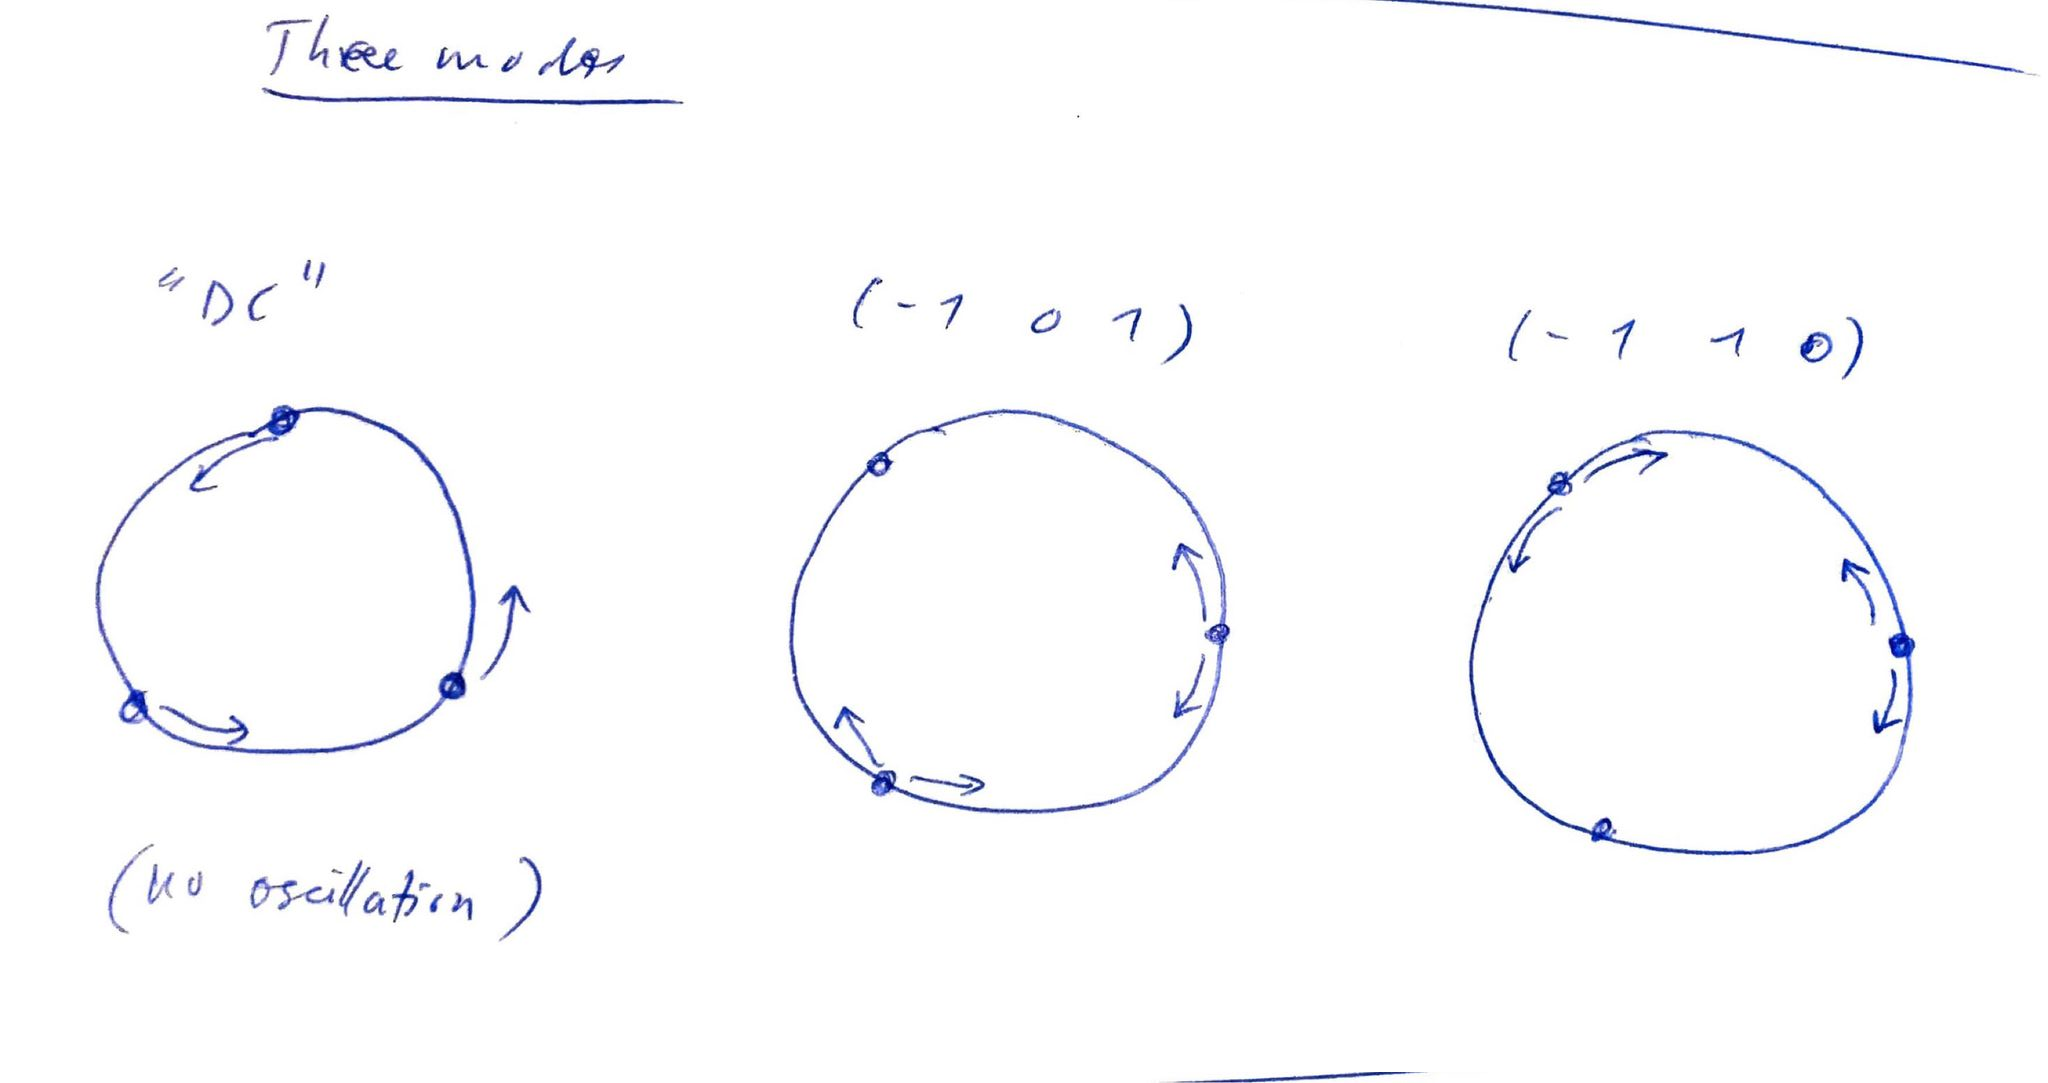
\includegraphics[width=0.75\textwidth]{modees1.jpg}
	\end{figure}
	
	
	
	\item Since $\omega_1 = 0$ and $\omega_2=\omega_3$, let us call $\omega_2 = \omega_3 = \Omega$ and simplify the general solution: 
	\begin{align*}
	\begin{pmatrix}
	\theta_1(t)\\
	\theta_2(t)\\
	\theta_3(t)
	\end{pmatrix}=
	\begin{pmatrix}
	A\cos\delta_1 - B\cos(\Omega t + \delta_2) - C\cos(\Omega t + \delta_3)\\
	A \cos\delta_1 + C\cos(\Omega t + \delta_3) \\
	A \cos\delta_1 + B\cos(\Omega t + \delta_2)
	\end{pmatrix}
	\end{align*}
	where $A,B,C,\delta_1,\delta_2,\delta_3$ are real numbers. With $\theta_1(0) = \theta_2(0) = \theta_3(0) = 0$ we have
	\begin{align*}
	\begin{pmatrix}
	A\cos\delta_1 - B\cos\delta_2 - C\cos\delta_3 \\
	A\cos\delta_1+C\cos\delta_3 \\
	A\cos\delta_1+B\cos\delta_2
	\end{pmatrix}
	= \begin{pmatrix}
	0\\0\\0
	\end{pmatrix}.
	\end{align*}
	This means $A\cos\delta_1 = 0 \implies C\cos\delta_3 = B\cos\delta_2 = 0$. So, the initial phases $\delta_2 = \delta_3 = \pi/2$. Next, with $\dot\theta_1(0) = -2\dot\theta_2(0) = -2\dot\theta_3(0) = 2\omega_0$ we have
	\begin{align*}
	\begin{pmatrix}
	\Omega (B\sin\delta_2 + C\sin\delta_3) \\ 
	-\Omega C\sin\delta_3 \\
	-\Omega B\sin\delta_2  
	\end{pmatrix}
	=
	\begin{pmatrix}
	\Omega(B+C)\\ -\Omega C \\ -\Omega B
	\end{pmatrix}
	=
	\begin{pmatrix}
	2\omega_0 \\-\omega_0 \\ -\omega_0
	\end{pmatrix}.
	\end{align*}
	So, $B=C= \omega_0/\Omega$.  Since $A\cos\delta_1 = 0$ we may ignore this first normal mode. The solution is 
	\begin{align*}
	\boxed{\begin{pmatrix}
	\theta_1(t)\\
	\theta_2(t)\\
	\theta_3(t)
	\end{pmatrix}=
	\f{\omega_0}{\Omega}\begin{pmatrix}
	-2\\
	1 \\
	1
	\end{pmatrix} \cos(\Omega t + \pi/2) = \f{\omega_0}{\Omega}\begin{pmatrix}
	2\\
	-1 \\
	-1
	\end{pmatrix} \sin(\Omega t)}
	\end{align*}
	
\end{enumerate}





\noindent \textbf{3. Small Oscillations of the Double Pendulum.} 
\begin{enumerate}[label=(\alph*)]
	\item Recall from Problem Set \#1 the kinetic and potential energies:
	\begin{align*}
	T 
	&= \f{1}{2}m_1 l_1^2 \dot\theta_1^2 + \f{1}{2}m_2 \lb l_1^2 \dot\theta_1^2 + l_2^2\dot\theta_2^2 + 2l_1l_2 \dot\theta_1 \dot\theta_2\cos(\theta_1-\theta_2)   \rb \\
	&= ml_1^2\dot\theta_1^2 + \f{1}{2}m l_2^2\dot\theta_2^2 + ml_1l_2\dot\theta_1\dot\theta_2\cos(\theta_1-\theta_2).
	\end{align*}
	The potential energy is 
	\begin{align*}
	V &= -(m_1+m_2)gl_1\cos\theta_1 - m_2 g l_2 \cos\theta_2\\
	&= -2m gl_1\cos\theta_1 - m gl_2\cos\theta_2.
	\end{align*}
	
	Under the small angle approximation $\cos\theta_1 \approx \cos\theta_2 \approx 1$ and $\cos(\theta_1-\theta_2) \approx \cos\theta_1\cos\theta_2 \approx 1$, we have 
	\begin{align*}
	T\approx ml_1^2\dot\theta_1^2 + \f{1}{2}m l_2^2\dot\theta_2^2 + ml_1l_2\dot\theta_1\dot\theta_2
	\end{align*}
	and up to second order in $\theta_1$ and $\theta_2$:
	\begin{align*}
	V &\approx -mg(2l_1+l_2) + \f{1}{2}mg l_2\theta_2^2 + mgl_1\theta_1^2\\
	&= \f{1}{2}mg [-2(2l_1+l_2) + 2l_1\theta_1^2 + l_2\theta_2^2].
	\end{align*}
	
	\item We Part (a), we see that 
	\begin{align*}
	\hat T = \begin{pmatrix}
	2ml_1^2 & ml_1l_2 \\ ml_1l_2 &ml_2^2
	\end{pmatrix}
	\end{align*}
	and 
	\begin{align*}
	\hat V = \begin{pmatrix}
	2mg l_1 & 0 \\ 0 & mgl_2
	\end{pmatrix}
	\end{align*}
	Solving $\det(\hat V - \omega^2 \hat T) = 0$ gives
	\begin{align*}
	\omega^2 = \f{g}{l_1l_2} \lb (l_1+l_2) \pm \sqrt{l_1^2 + l_2^2} \rb
	\end{align*}
	Notice that $(l_1+l_2)^2 \geq l_1^2 + l_2^2$, so both solutions are valid. From here, we find two (real and positive) normal frequencies:
	\begin{align*}
	\boxed{\omega_+ = \sqrt{\f{g}{l_1l_2} \lb (l_1+l_2) + \sqrt{l_1^2 + l_2^2} \rb} 
	\quad\quad 
	\omega_- = \sqrt{\f{g}{l_1l_2} \lb (l_1+l_2) - \sqrt{l_1^2 + l_2^2} \rb}}
	\end{align*}
	
	\item The corresponding eigenvectors are
	\begin{align*}
	\boxed{\epsilon_+ = \f{1}{2l_1}\begin{pmatrix}
	 (l_1-l_2) - \sqrt{l_1^2 + l_2^2}  \\ 2l_1
	\end{pmatrix} 
	\quad\quad 
	\epsilon_- = \f{1}{2l_1}\begin{pmatrix}
	(l_1-l_2) + \sqrt{l_1^2 + l_2^2}  \\ 2l_1
	\end{pmatrix}} 
	\end{align*}
	The normal modes are thus
	\begin{align*}
	&\boxed{\vec{\eta}_+ = \f{1}{2l_1}\begin{pmatrix}
	(l_1-l_2) - \sqrt{l_1^2 + l_2^2}  \\ 2l_1
	\end{pmatrix} \exp\lb it\sqrt{\f{g}{l_1l_2} \lb (l_1+l_2) + \sqrt{l_1^2 + l_2^2} \rb}\rb e^{i\delta_1}}\\
	&\boxed{\vec{\eta}_- = \f{1}{2l_1}\begin{pmatrix}
	(l_1-l_2) + \sqrt{l_1^2 + l_2^2}  \\ 2l_1
	\end{pmatrix} \exp\lb it\sqrt{\f{g}{l_1l_2} \lb (l_1+l_2) - \sqrt{l_1^2 + l_2^2} \rb}\rb e^{i\delta_2}}
	\end{align*}
	To simplify computations, we shall let $\mu = l_2/l_1$, the ratio of the rod lengths. With this, the eigenvalues and normal modes become 
	\begin{align*}
	\omega_\pm = \sqrt{\f{g}{l_2}} \sqrt{ 1 + \mu \pm \sqrt{1+\mu^2}}
	\end{align*}
	and
	\begin{align*}
	\vec{\eta}_\pm = \f{1}{2}\begin{pmatrix}
	1-\mu \mp \sqrt{1+\mu^2} \\ 2 
	\end{pmatrix}  e^{i\omega_\pm t} e^{i\delta_1}.
	\end{align*}
	Call $\kappa_\pm = \mu \pm \sqrt{1+\mu^2}$. Then 
	\begin{align*}
	\omega_\pm = \sqrt{\f{g}{l_2} ( 1 + \kappa_\pm) }
	\end{align*}
	and
	\begin{align*}
	\vec{\eta}_\pm = \f{1}{2}\begin{pmatrix}
	1-\kappa_\pm \\ 2 
	\end{pmatrix}  e^{i\omega_\pm t} e^{i\delta_1}.
	\end{align*}
	
	Sketch: We may consider two limits: $\mu \approx 0,1,\infty$. If $\mu \approx \infty$ then the fast oscillation $\omega_+$ becomes unimportant and what's left is the slow solution $\omega_- \approx \sqrt{g/l_2}$. This is just simple harmonic motion for $m_2$. If $\mu \approx 0$ then the fast oscillation $\omega_-$ becomes unimportant and what's left is the slow solution $\omega_+ \approx \sqrt{g/l_1}$ which is just simple harmonic motion for $(m_1+m_2)$. The interesting limit is where $\mu \approx 1$. This is where we will see the normal modes. In this case, $\kappa_\pm \approx 1\pm\sqrt{2}$, and so $1-\kappa_\pm = \mp \sqrt{2}$. So the fast solution is one where the masses oscillate in opposite directions, while the slow solution is one where the masses oscillate in the  same direction. 
	
	\textcolor{red}{Sketch:}
	\begin{figure}[!htb]
		\centering
		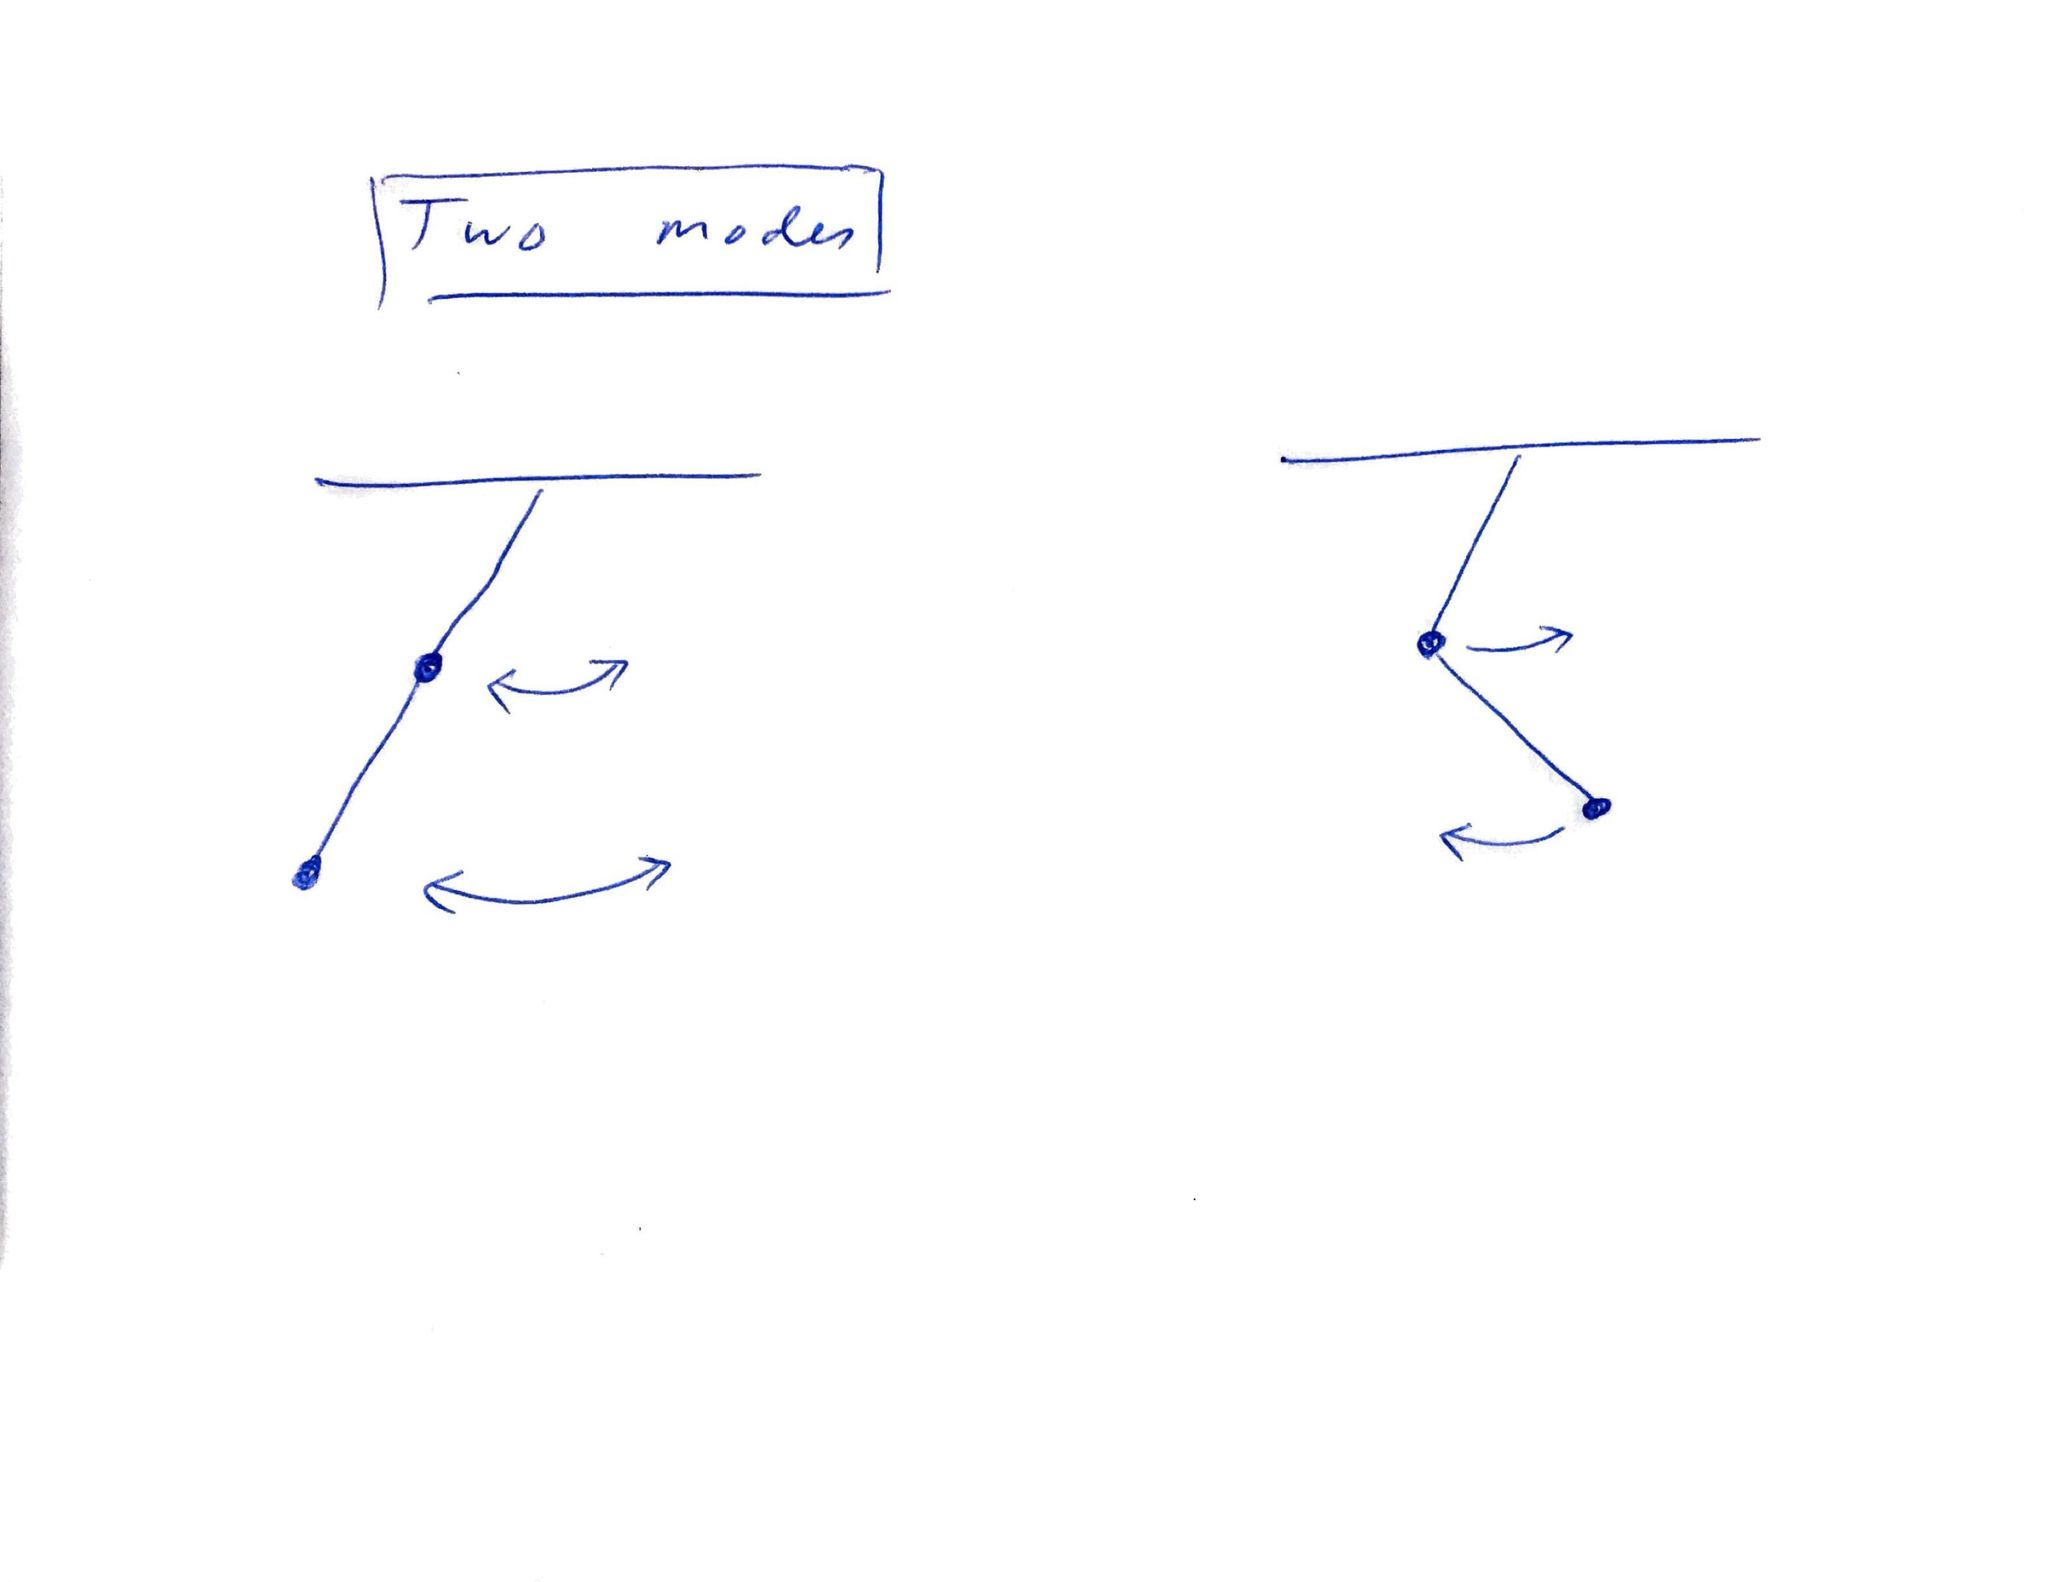
\includegraphics[width=0.75\textwidth]{modes2}
	\end{figure}
	
\end{enumerate}

\newpage

\noindent \textbf{4. A Rigid Oscillating Bar.} [8.09 ONLY] \\


\noindent \textbf{5. A Rigid Oscillating Bar.} Pick our coordinates to be $(x_\text{CM}, y_\text{CM}, \phi)$ where $(x_\text{CM},y_\text{CM})$ is the center-of-mass position of the rod, and $\phi$ is the tilt of the rod from the horizontal. Let $y=0$ to be the ``ceiling.'' To begin this problem, we first have to work out all the relevant geometrical factors. First is the position of the anchor points. At equilibrium, the distance between the anchor points for the springs is 
\begin{align*}
2\lambda = L +2 a\sin\theta_0. 
\end{align*}
And so the anchor positions are $r_- = -(L/2 + a\sin\theta_0,0)$ and $r_+ = (L/2+a\sin\theta_0,0)$. More compactly, 
\begin{align*}
r_\pm = \pm (l+a\sin\theta_0,0) = (\pm \lambda,0).
\end{align*}



\begin{enumerate}[label=(\alph*)]
	\item
	
	
	
	
	
	
	The kinetic energy is rather straightforward. The relevant moment of inertia is $i = mL^2/12$.
	\begin{align*}
	T = \f{1}{2}m (\dot{x}_\text{CM}^2 + \dot{y}_\text{CM}^2) + \f{1}{2}\f{1}{12}mL^2\dot\phi^2.
	\end{align*}
	The potential energy is the sum of the gravitational potential and the energy stored in the springs. Let the natural length of the springs be $a_0$. To find $a_0$, we use Newton's law. At equilibrium, the rod does not accelerate, so the force due to the springs and gravity cancel. So,
	\begin{align*}
	mg = 2k(a-a_0)\cos\theta_0.
	\end{align*}
	So the natural length of each spring is 
	\begin{align*}
	\boxed{a_0 = a- \f{mg}{2k\cos\theta_0}}
	\end{align*}
	
	
	
%	we must find $y_0$. By conservation of energy, the increase in gravitational potential energy is the decrease in spring potential:
%	\begin{align*}
%	(a\cos\theta_0 - y_0)mg = 2\f{1}{2}k(a - a_0)^2 = k(a-a_0)^2 \implies y_0 = a\cos\theta_0 - \f{k}{mg}(a-a_0)^2.
%	\end{align*}
%	Plugging this into the first equation lets us solve for $a_0$. \textcolor{blue}{This is ugly so I won't do it for now. Or maybe I'm approaching this incorrectly. In any case, 
	
	
	
	The natural lengths of the springs don't matter in the end, so we won't write them out explicitly. The potential energy is
	\begin{align*}
	V = -mgy_\text{CM} + \f{1}{2}k(l_- -a_0)^2 + \f{1}{2}k(l_+-a_0)^2.
	\end{align*}
	We need to find the lengths $l_\pm$ of the springs (left/right, respectively). $l_+$ is the distance between the right anchor point and the right tip of the rod $\vec{R}_\pm = (x_\text{CM} \pm l\cos\phi, y_\text{CM}\pm l\sin\phi)$:
	\begin{align*}
	l_\pm 
	&= \abs{\vec{r}_\pm - \vec{R}_\pm }\\
	&= \sqrt{[\pm \lambda - (x_\text{CM} \pm l\cos\phi)]^2 + (y_\text{CM} \pm l\sin\phi)^2}\\
	&= \sqrt{[\pm (l+a\sin\theta_0) - (x_\text{CM} \pm l\cos\phi)]^2 + (y_\text{CM}\pm l\sin\phi)^2}.
	\end{align*}
	With this, the potential energy is 
	\begin{align*}
	V = -mgy_\text{CM} + \f{1}{2}k\lb \sqrt{[- (l+a\sin\theta_0) - (x_\text{CM} - l\cos\phi)]^2 + (y_\text{CM}- l\sin\phi)^2} -a_0\rb^2 \\
	+ \f{1}{2}k\lb 
	\sqrt{[(l+a\sin\theta_0) - (x_\text{CM} + l\cos\phi)]^2 + (y_\text{CM}+ l\sin\phi)^2}   -a_0\rb^2.
	\end{align*}
	The Lagrangian is just the difference between $T$ and $V$: $\lag = T-V$. I won't write it out here. 
	
	
	\item For simplicity, we shall work with the following coordinates $(x,y,\Phi)$ where 
	\begin{align*}
	x = x_\text{CM} \quad\quad y = y_\text{CM} - a\cos\theta_0 \quad\quad \Phi = L\phi/2 = l\phi.
	\end{align*}
	where $a\cos\theta_0$ is the equilibrium vertical position. Consider small amplitude oscillations. We then see that $x,y,\Phi$ are small.  We may also assume, as suggested by the problem, that $\theta_0$ is small. The kinetic energy is 
	\begin{align*}
	T = \f{1}{2}m (\dot{x}^2 + \dot{y}^2) + \f{1}{2}\f{1}{3}m\dot\Phi^2
	\end{align*}
	which gives
	\begin{align*}
	\boxed{\hat T = m\begin{pmatrix}
	1 & 0 & 0 \\
	0 & 1 & 0 \\
	0 & 0 & 1/3
	\end{pmatrix}}
	\end{align*}
	To find a nice form for $V$, we must apply the small amplitude approximation to the spring lengths $l_\pm$:
	\begin{align*}
	l_\pm  
	&= \sqrt{[\pm \lambda - (x_\text{CM} \pm l\cos\phi)]^2 + (y_\text{CM} \pm l\sin\phi)^2}\\
	&\approx \sqrt{[\pm \lambda - (x \pm l)]^2 + (y + a\cos\theta_0 \pm \Phi)^2}\\
	&= \lb \lambda^2 \mp 2\lambda(x\pm l)+(x\pm l)^2 + (y + a\cos\theta_0\pm \Phi)^2 \rb^{1/2}\\
	&= \lb (\lambda^2 + l^2 - 2l\lambda) + \cancel{x^2} \mp 2(\lambda-l) x + (y + a\cos\theta_0\pm \Phi)^2 \rb^{1/2}\\
	&= \lb (\lambda- l)^2 \mp 2(\lambda-l) x + (y + a\cos\theta_0\pm \Phi)^2 \rb^{1/2}\\
	&\approx \lb (\lambda- l)^2 \mp 2(\lambda-l) x
	+ (y+a\cos\theta_0)^2 \pm 2\Phi(y+a\cos\theta_0) + \cancel{\Phi^2} \rb^{1/2} \\
	&\approx \lb (\lambda- l)^2 \mp 2(\lambda-l) x  + \cancel{y^2} + 2ya\cos\theta_0 +a^2\cos^2\theta_0 \pm \cancel{2\Phi y} \pm 2\Phi a\cos\theta_0  \rb^{1/2}.
	\end{align*}
	Before we proceed, we observe that $a^2 = (\lambda-l)^2 + (a\cos\theta_0)^2 = a^2\sin^2\theta_0 + a^2\cos^2\theta_0 $ due to the geometry of the problem. Thus, we may factor out $a$. 
	\begin{align*}
	l_\pm 
	&\approx a \lb 1 \mp \f{2(\lambda-l) x}{a^2} + \f{2y\cos\theta_0}{a} \pm \f{2\Phi \cos\theta_0}{a} \rb^{1/2}\\
	&\approx a\lb 1 \mp \f{(\lambda-l) x}{a^2}  + \f{y\cos\theta_0}{a} \pm \f{\Phi\cos\theta_0}{a} \rb.
	\end{align*}
	Next, since we have
	\begin{align*}
	\sin\theta_0 = \f{\lambda-l}{a}, \quad\quad \cos\theta_0 = \f{a\cos\theta_0}{a},
	\end{align*}
	and small $\theta_0$, we may ignore that term $\lambda\Phi/a^2$ as well and write
	\begin{align*}
	l_\pm \approx a \mp x \sin\theta_0 + y\cos\theta_0 \pm \Phi \cos\theta_0.
	\end{align*}
	We may now plug $l_\pm$ into $V$:
	\begin{align*}
	V 
	&= -mgy_\text{CM} + \f{1}{2}k(l_- -a_0)^2 + \f{1}{2}k(l_+-a_0)^2\\
	&\approx -mg(y+a\cos\theta_0) + \f{k}{2}\lb a + x \sin\theta_0 + y\cos\theta_0 - \Phi \cos\theta_0 -a_0 \rb^2\\
	&\quad\quad + \f{k}{2}\lb a - x \sin\theta_0 + y\cos\theta_0 + \Phi \cos\theta_0 - a_0\rb^2\\
	&\approx \text{constants } + \text{ linear terms } + k\lb x^2\sin^2\theta_0 + y^2\cos^2\theta_0
	+ \Phi^2\cos^2\theta_0 - 2x\Phi \sin\theta_0\cos\theta_0\rb.
	\end{align*}
	With this we find 
	\begin{align*}
	\boxed{\hat V = 
	2k\begin{pmatrix}
	\sin^2\theta_0 & 0 & -\sin\theta_0 \cos\theta_0 \\
	0 & \cos^2\theta_0 & 0  \\
	-\sin\theta_0 \cos\theta_0 & 0 & \cos^2\theta_0
	\end{pmatrix}}
	\end{align*}
	
	
	
	
	
	
	
	
	\item We will save the small angle approximation on $\hat{V}$ for later. Now, solving $\det(\hat{V} - \omega^2 \hat{T}) = 0$ gives
	\begin{align*}
	{\omega_1^2 = 0 \quad\quad \omega_1^2 = \f{2k\cos^2\theta_0}{m} \quad\quad \omega_2^2 = \f{2k(2+\cos2\theta_0)}{m}}
	\end{align*}
	Using Mathematica we may find the eigenvectors:
	\begin{align*}
	\vec{a}_1 = \begin{pmatrix}
	\cos\theta_0 \\ 0 \\ \sin\theta_0
	\end{pmatrix};
	\quad 
	\vec{a}_2 = \begin{pmatrix}
	0 \\ 1 \\ 0
	\end{pmatrix}; \quad
	\vec{a}_3 = \begin{pmatrix}
	-\sin\theta_0 \\ 0 \\ 3\cos\theta_0
	\end{pmatrix}
	\end{align*}
	So the normal modes are 
	\begin{align*}
	\boxed{\vec{\eta}_1 \propto \begin{pmatrix}
	\cos\theta_0 \\ 0 \\ \sin\theta_0
	\end{pmatrix}\approx \begin{pmatrix}
	1 \\ 0 \\ \theta_0
	\end{pmatrix}; \quad
	\vec{\eta}_2 \propto \begin{pmatrix}
	0 \\ 1 \\ 0
	\end{pmatrix} e^{i\omega_2 t}; \quad 
	\vec{\eta}_3 \propto \begin{pmatrix}
	-\theta_0 \\ 0 \\ 3
	\end{pmatrix}e^{i\omega_3 t}}
	\end{align*}
	When $\theta_0 = 0$, then we see that the motions in $x,y,\Phi$ in the normal modes are completely decoupled. In the first normal mode, we only have oscillations in the $x$ direction. In the third normal mode, we only have oscillation about the equilibrium position of the center of mass. The second normal mode is unaffected. The frequencies of the second and third normal modes are $\sqrt{2k/m}$ and $\sqrt{6k/m}$, respectively. The first normal mode is still ``DC.''	
	\newpage
	
	\textcolor{red}{Sketch:}
	\begin{figure}[!htb]
		\centering
		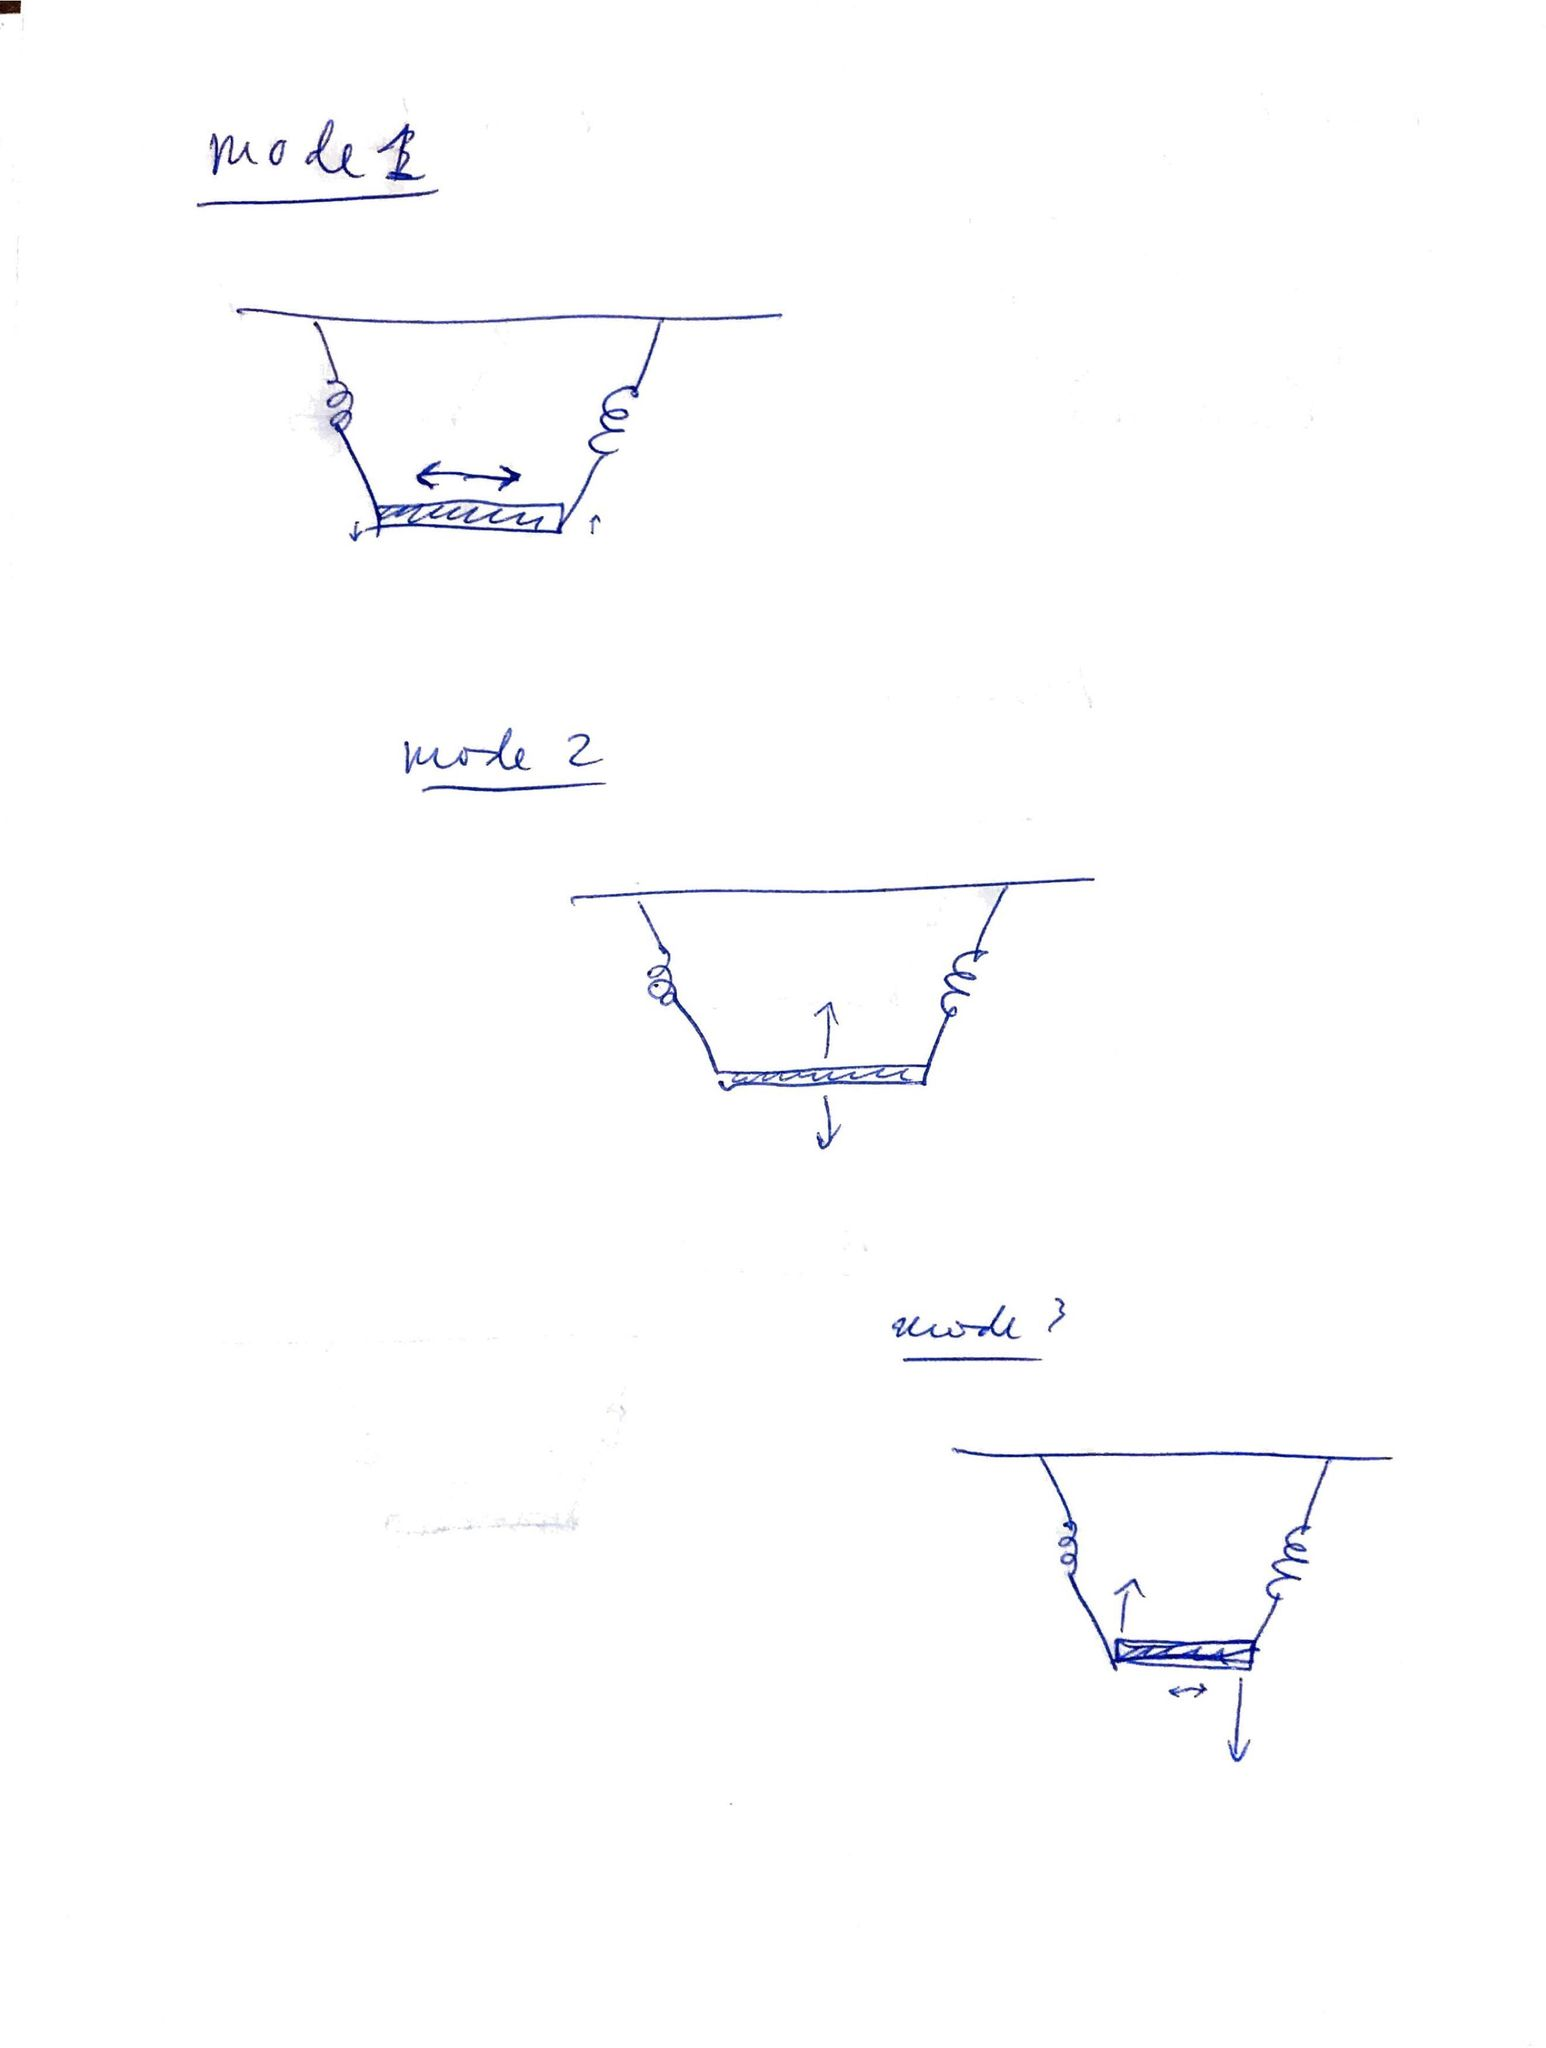
\includegraphics[width=0.75\textwidth]{modes5}
	\end{figure}
	
\end{enumerate}

	
\end{document}



